\documentclass{standalone}
\usepackage{tikz}
\usetikzlibrary{backgrounds,fit,shapes.geometric}

\begin{document}
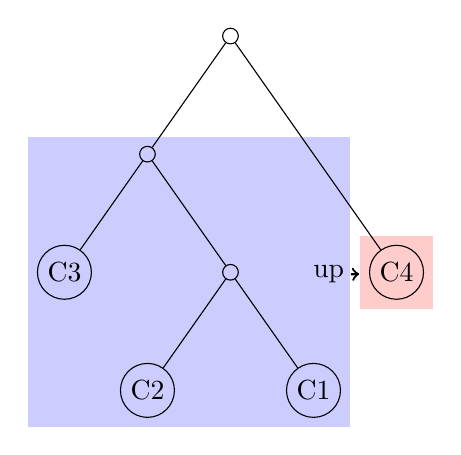
\begin{tikzpicture}[sibling distance=60pt, every node/.style={inner sep=2pt, circle, draw}]
\node (site) {}
  child { node (CP1) {}
    child { node (C3) {C3} }
    child { node (CP2) {}
      child { node (C2) {C2} }
      child { node (C1) {C1} }
    }
  }
  child { coordinate {} child[missing]  child { node (C4) {C4} } };

  \begin{scope}[on background layer, every node/.style={rectangle, draw=none}]
    \node[fill=red!20, fit=(C4)] (CV1) {};
    \node[fill=blue!20, fit=(CP1) (C3) (C2) (C1)] (here) {};
  \end{scope}
  \draw[->, thick] (here) -- node[draw=none, left] {up} (CV1);
\end{tikzpicture}\hfill
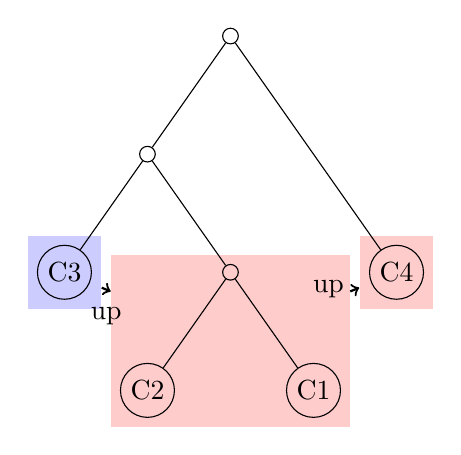
\begin{tikzpicture}[sibling distance=60pt, every node/.style={inner sep=2pt, circle, draw}]
\node (site) {}
  child { node (CP1) {}
    child { node (C3) {C3} }
    child { node (CP2) {}
      child { node (C2) {C2} }
      child { node (C1) {C1} }
    }
  }
  child { coordinate {} child[missing]  child { node (C4) {C4} } };

  \begin{scope}[on background layer, every node/.style={rectangle, draw=none}]
    \node[fill=red!20, fit=(C4)] (CV1) {};
    \node[fill=red!20, outer sep=0pt, fit=(CP2) (C2) (C1)]
    (CV2) {};
    \node[fill=blue!20, rectangle, fit=(C3)] (here) {};
  \end{scope}
  \draw[->, thick] (CV2) -- node[draw=none, left] {up} (CV1);
  \draw[->, thick] (here) -- node[draw=none, below] {up} (CV2);
\end{tikzpicture}\hfill
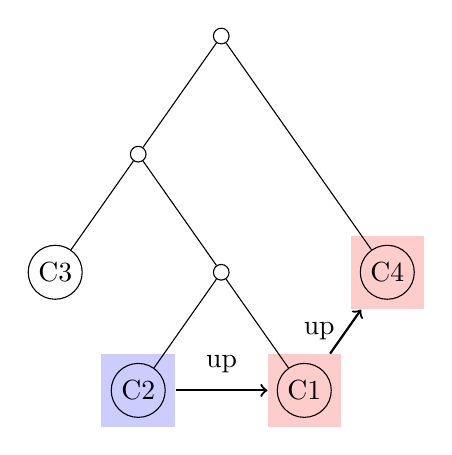
\begin{tikzpicture}[sibling distance=60pt, every node/.style={inner sep=2pt, circle, draw}]
\node (site) {}
  child { node (CP1) {}
    child { node (C3) {C3} }
    child { node (CP2) {}
      child { node (C2) {C2} }
      child { node (C1) {C1} }
    }
  }
  child { coordinate {} child[missing]  child { node (C4) {C4} } };

  \begin{scope}[on background layer, every node/.style={rectangle, draw=none}]
    \node[fill=red!20, fit=(C4)] (CV1) {};
    \node[fill=red!20, outer sep=0pt, fit=(C1)] (CV2) {};
    \node[fill=blue!20, rectangle, fit=(C2)] (here) {};
  \end{scope}
  \draw[->, thick] (CV2) -- node[draw=none, left] {up} (CV1);
  \draw[->, thick] (here) -- node[draw=none, above] {up} (CV2);
\end{tikzpicture}
\end{document}
